\chapter{Ein Anhangskapitel}

Hier könnte ein Anhang stehen, falls Sie z.\,B.\ Code, Konstruktionszeichnungen oder Ähnliches mit in die Arbeit bringen wollen.
Im Normalfall stehen jedoch alle Ihre Resultate im Hauptteil der Bachelorarbeit und ein Anhang ist überflüssig.

\section{Einkristalloberflächen}
        Die geordneten Strukturen eines Einkristalls kommen durch die Wechselwirkung der Elektronen zwischen den einzelnen Atomen.
        So ergibt sich eine periodische Anordnung der Atome im thermischen Gleichgewicht.
        Dabei sind die Atome nicht komplett starr an ihre Plätze gebunden, sondern führen kleine Schwingungen um diesen aus.
        Mit der Temperatur sinkt auch die Auslenkung.
        Dieses Wechselspiel der strukturellen Ordnung findet sich auch in der elektronischen Struktur wieder.
                
        Wird ein Einkristall entlang einer Kristalleben durchschnitten so ergibt sich eine Oberfläche.
        Die Ebene erhält den Namen der Indizes des auf ihr senkrecht stehenden Gittervektors $r_{hkl}$, also $(hkl)$.
        Als Oberfläche werden die oberen Atomlagen definiert, die sich in der geometrischen und/oder chemischen Art von der des Volumens unterscheiden~\cite{Fauster}.
        Aufgrund der nun fehlenden Bindungen nach oben ergeben sich neue elektronische und geometrische Eigenschaften.
        So kann es zu lateralen und transversalen Verschiebungen gegenüber der volumenartigen Struktur, so genannte Rekonstruktionen und Relaxation kommen.
        Dabei ordnen sich die Atome um, um damit einen energetisch günstigeren Zustand zu erhalten.
    
        Wie im Volumenkristall kann die Oberfläche durch eins von fünf Bravais-Gittern beschrieben werden, wobei auf jedem Gitterpunkt eine atomare Basis gesetzt wird.
        Die Punkte dieses zweidimesionalen Gitters lassen sich durch den Gittervektor
        \begin{equation}
            \vec{r}_{nm} = n \vec{a}_1 + m \vec{a}_2
            \label{eqn:Gittervek}
        \end{equation}
        mit $n,m \in \mathbb{Z}$ und den Vektoren der Einheitszelle $\vec{a}_1, \vec{a}_2$ beschreiben.
        Geimeinsam legt das Bravais-Gitter und die atomare Basis die Symmetrien der Oberfläche fest.
    
        Durch die Anlagerung von Adsorbaten können Symmetrien der Oberfläche verloren gehen.
        Die Struktur der Adsorbate relativ zur Oberfläche wird Überstruktur genannt.
        Durch den meist größeren Abstand der Adsorbate untereinander als der Basen des Substrates ergibt sich auch eine größere Einheitszelle.
        Beim Schneiden der Einkristalle um eine Oberfläche zu erhalten können sich unter anderem auch Stufen ausbilden.
        Vermehrt treten diese Stufen bei hochindizierten Oberflächen auf, wobei einzelne Terrassen dann eine niedrigindizierte Oberfläche darstellen~\cite{Fauster}.
        Diese Stufen oder auch Defekte in der Oberfläche bilden Keimzellen für Anlagerung von Adsorbaten.
        Um die Überstruktur des Adsorbate zu beschreiben wird die von ihnen aufgespannte Einheitszelle aus den Gittervektoren des Substrats rekosntruiert.
        Die Gittervektoren des Übergitters $\vec{b}_1, \vec{b}_2$ lassen sich dann als Matrixschreibweise darstellen.
        Damit ergibt sich auch die Überstrukturmatrix $C$ mit 
        \begin{equation}
            \begin{pmatrix}
                \vec{b}_1 \\
                \vec{b}_2 \\
            \end{pmatrix}
            = 
            \begin{pmatrix}
                C_{11} & C_{12} \\
                C_{21} & C_{22} \\
            \end{pmatrix}
            \begin{pmatrix}
                \vec{a}_1 \\
                \vec{a}_2 \\
            \end{pmatrix}.
        \end{equation}
        Relative Verschiebungen zum Substrat bleiben dabei ohne Beachtung, es zeigt nur die Periodizität der Struktur an.
        Ferner kann es zur Aubildung verschiedener Domänen kommen, besonders dann, wenn die Symmetrie des Übergitters kleiner als die des Substrates ist~\cite{Fauster}.
        Einzelne Domänen weisen Symmetrie äquivalente Anordnungen auf, häufug handelt es sich nur umgedrehte Einheitszellen.
        Nicht nur Adsorbatebedeckungen lassen sich durch diese Notation beschreiben, auch die Rekonstruktion der Oberfläche.
        Hierbei sind es keine Adsorbatatome, sondern die Oberflächenatome selbst, die eine neue Struktur ausbilden.
        Die Relaxation, welche die Änderung im Lagenabstand beschreibt kann hingegen nicht durch dies Notation beschrieben werden.
        Sie ist ebenso wie die Rekonstruktion vom Material, der Kristallstruktur und der Oberflächenorientierung abhängig.
        Einige Rekonstruktionen und Relaxation hängen auch vom Präperationsprozess ab, wenn die Oberfläche selbst metastabil ist.
    
        Wie bereits erwähnt hängen geometrische und elektronische Struktur stark zusammen.
        Sodass sich an Oberflächen durch die fehlenden Bindungen die elektronische Struktur verändern kann.
        Die quantenmechanische Beschreibung der Elektronen erlaubt es auch die elektronischen Zustände der Oberfläche durch Quantenzahlen auszudrücken.
        Hier ist $\vec{k}_{||}$ der Wellenzahlvektor der Oberfläche die Ausschlag gebende Größe um die Oberflächenbandstruktur $E(\vec{k}_{||})$ zu beschreiben.
        Ganz besondere Beachtung erhalten die Zustände nahe der Fermikante $E_\text{F}$ die für leitenden Eigenschaften verantwortlich sind.
        Erhaltene Oberflächenbandstruktur kann von der der Volumenbandstruktur abweichen.
        Dies führt zum Teil zu Oberflächenzuständen, die unterscheiden sich energetisch von denen im Volumenkristall und können somit nur in dessen Bandlücke auftreten.
    
        % Ein wichtiger Ansatz für die periodische Struktur der Oberfläche und dessen elektronischen Zustände ist das Bloch Theorem.
        % Die Oberfläche entspricht einer Anordung äquivalenter Punkte welche durch den Gittervektor aus \autoref{eqn:Gittervek} ineinander überführt werden können

    \section{TMOS}    
    \begin{itemize}
        \item Symmetriebrechung, Verspannung (WW mit Substrat), Polarität, Filmdicke, Kristallograpische Orientierung
        \item Verständnis ist wichtig um Phasenübergänge durch gezielten Doping, Temperatur oder äußeres Magnetfeld für die Anwendung nutzbar zu machen
        \item Magnetische Widerstandsänderung erläutern? (GMR, TMR, CMR)
        \item Vor allem in dem \ce{Fe3O4} in dem das Eisen als (2+) und (3+) Ion auf unterschiedlichen Gitterplätzen (tetraedisch oder oktaedrisch) vorkommt, kommt es zu unterschiedlichen Aufspaltungen der $e_g$ und $t_{2g}$ Energieniveaus.
    \end{itemize}

    \section{Eisen (100) Oberfläche}
        \begin{itemize}
            \item WKF
            \item Symmetrie - p4mm
            \item Gitterkonstante ist $a = \SI{2.862}{\angstrom}$~\cite{springer_database}
            \item bcc Struktur
        \end{itemize}
    
    \section{Gold (111) Oberfläche}
        Gold gehört zu den Edelmetallen und kristallisiert in der flächenzentrierten Struktur mit einer Gitterkonstanten von \SI{4.08}{\angstrom}~\cite{Marx}.
        Es ist besonders leitfähig, stabil und wenig reaktiv, dennoch rekosntruiert die Oberfläche in einer Fischgräten-Struktur ($\num{22} \times \sqrt{\num{3}}$)~\cite{5A_3}.
        Die Austrittsarbeit der (111)-Oberfläche wurde dabei auf \SI{5.46}{\electronvolt} bestimmt~\cite{5A_4}.
        Ebenfalls bildet sich auch ein sehr präsenter Oberflächenzustand aus.
        
        Auf Grund der sehr ähnlichen Gitterkonstante zu der des Nickeloxids von nur etwa \SI{2}{\percent} eignet es sich besonders gut als Substrat \cite{NiO_36}.
        \begin{itemize}
            \item Ebenenabstand in Au(111) $d_0 = \SI{2.35}{\angstrom}$.\textbf{\cite{5A_1}}
        \end{itemize}
        Bereits bekannt ist, dass sich auf diesem Substrat das Pentacene anordnet~\cite{5A_1, 5A_3}.
        Die lange Molekülachse liegt dabei parallel zu den Reihen der Goldatome, mit den äußeren Ringen und somit die $\pi$-Orbitale direkt oberhalb eines Goldatoms.
        Diese Positionierung lässt auf eine starke Substrat-Molekül-Interaktion schließen~\cite{5A_3}.
        Bei der Wechselwirkung dieser handelt es sich um Physisorption, was damit auch die Adsorbate-Adsorbat-Wechselwirkung zur Formung der Einheitszelle dominieren lässt~\cite{5A_4}.
        Ferner liegen in einer Monolage flach auf der Oberfläche und einzelne Reihen sind durch eine Reihe Goldatome separiert.
        Allerdings wächst der Pentacenefilm nicht epitaxtisch, sondern in Form von Inseln mit unterschiedlichen Einheitszellen~\cite{5A_3}.
        \begin{figure}
            \centering
            \includegraphics[width=0.5\textwidth]{Au+5A/EDC_Au_5A_mod.png}
            \caption{Die integrierten Spektren für reines Gold, Gold mit einer Monolage Pentacene und deren Differenz.}
            \label{fig:EDC_Au+5A}
        \end{figure}
        Das Goldsubstrat eignet sich ebenfalls zur Kalibrierung der Monolage von Pentacene, da bereits bekannt ist, dass sich diese flach auf der Oberfläche ordnet \cite{5A_1}.
        Bei der Wechselwirkung mit dem Substrat handelt es sich um die Physisorption durch einen Substrat-Molekülabstand von \SI{3.28}{\angstrom} \cite{5A_1}.
        % Es ergibt sich so das LEED-Bild in \autoref{fig:LEED_Au+5A}, was auch die bekannte \textbf{Überstruktur} (5A_1, 5A_5) aufweist.
        Schaut man sich das winkelintegrierte Spektrum im Bereich der Valenzzustände in \autoref{fig:EDC_Au+5A} an, so sind auch deutlich Elemente zu erkennen, die durch die Moleküle hervorgerufen werden.
        Die senkrechten Linien stellen die Punkte da, an denen Bilder mit höherer Statistik aufgenommen wurden und die später zur Molekülorbitalanalyse herangezogen werden.

        \begin{figure}
            \centering
            \begin{subfigure}[t]{0.48\textwidth}
                \centering
                \includegraphics[height=4cm]{Au+5A/MOT_Au_5A_exp_1.png}
                \subcaption{Gemmesen, symmetrisiertes Bild bei einer Bindungsenergie von \SI{0.8}{\electronvolt}.}
                \label{fig:MOT_Au+5A_exp_1}
            \end{subfigure}
            \begin{subfigure}[t]{0.48\textwidth}
                \centering
                \includegraphics[height=4cm]{Au+5A/HOMO_all_CT}
                \subcaption{Das theoretisch erwartete HOMO.}
                \label{fig:MOT_Au+5A_theo_1}
            \end{subfigure}
            \centering
            \begin{subfigure}[t]{0.48\textwidth}
                \centering
                \includegraphics[height=4cm]{Au+5A/MOT_Au_5A_exp_2.png}
                \subcaption{Gemmesen, symmetrisiertes Bild bei einer Bindungsenergie von \SI{1.85}{\electronvolt}.}
                \label{fig:MOT_Au+5A_exp_2}
            \end{subfigure}
            \begin{subfigure}[t]{0.48\textwidth}
                \centering
                \includegraphics[height=4cm]{Au+5A/HOMO1_all_CT}
                \subcaption{Theorie Oribtale mit Symmetrisierung des HOMO-1.}
                \label{fig:MOT_Au+5A_theo_2}
            \end{subfigure}
            \begin{subfigure}[t]{0.48\textwidth}
                \centering
                \includegraphics[height=4cm]{Au+5A/MOT_Au_5A_exp_3.png}
                \subcaption{Gemmesen, symmetrisiertes Bild bei einer Bindungsenergie von \SI{2.65}{\electronvolt}.}
                \label{fig:MOT_Au+5A_exp_3}
            \end{subfigure}
            \begin{subfigure}[t]{0.48\textwidth}
                \centering
                \includegraphics[height=4cm]{Au+5A/HOMO2_all_CT}
                \subcaption{Berechnetes Theoriebild zum HOMO-2.}
                \label{fig:MOT_Au+5A_theo_3}
            \end{subfigure}
            \caption{Zuordnung eines Bildes zu einem der Molekülorbitale. Theorie Oribtale mit Symmetrisierung zweimal um 120 Grad gedreht und zum Ursprungsbild addiert.}
            \label{fig:MOT_Au+5A}
        \end{figure}
        Winkelaufgelöste Bilder bei den entsprechenden Energien zeigen auch zusätzliche Merkmale im Bezug zum reinen Gold.
        Gemeinsam mit theoretischen Berechnungen aus der Dichtefunktionaltheorie lassen sich diese dann entsprechenden Molekülorbitalen zuordnen.
        Dies ist für einige Energien und Orbitale in \autoref{fig:MOT_Au+5A} geschehen.
        Dabei wurden die gemessenen wie auch berechneten Bilder entsprechend der Geometrie aus dem Beugungsbild \autoref{fig:LEED_Au+5A} jeweils um \SI{120}{\degree} gedreht und aufsummiert.

        Eine Zuordnung einer der markanten Elemente zu einem zuvor unbestzten Orbital, dem LUMO ist nicht zu erkennen.
        Es scheint also so als würden keine Elektronen zwischen Substrat und Molekül ausgetauscht werden. 
        Dies lässt sich auch aus der Literatur erkennen, dass sich bei den Anornung von Pentacene auf Gold um den Prozess der Physisorption handelt~\cite{5A_4}.
        Abwesenheit des LUMOs in den Spektren und Bildern muss aber nicht zwangsläufig auf die Physisorption hindeuten.
        So ist Pentacene auf Kupfer (111) chemisch adsorbiert und zeigt dennoch keine Anzeichen der Besetzung des LUMO~\cite{koch_adsorption-induced_2008}.
            \section{Sonstiges}
            \begin{itemize}
                \item Die mittlere freie Weglänge $\lambda$ ist die in der \SI{63}{\percent} der Elektronen Energieverlust erfahren \cite{vickerman_surface_2009}
                \item Durch den Vergleich von VB bei XPS und UPS sieht man Effekt ob von metallischem d (XPS) oder Liganden kommt (UPS - Intensitäten gleich ob metalisch oder Ligand) \cite{FeO_44}
            \end{itemize}

            \subsection{XMCD/XMLD}
            Neben der Abhänigkeit von der Photonenenergien ist die Absorption auch von der Polarisation des Lichts selbst abhängig.
            So lässt sich aus den Unterschieden der Absorptionsintensitäten für s- und p-polarisiertem Licht die Neigung von Molekülen auf der Oberfläche kalkulieren\cite{floreano_periodic_2008}.
            Ebenso wird durch die Ausrichtung der magetischen Momente die Orbitalstruktur ebenfalls in diese Richtung gestreckt.
            Nun kommt der Polarisationfaktor für den Photoemissionsstrom zu tragen.
            Sind Polarisation der Photonen und Orbitalgeometrie parallel gerichtet kommt es zur verstärkten Absorption, im Gegensatzt dazu, wenn diese senkrecht aufeinander stehen.
            Aus der Differenz der beiden Anteile ergibt sich dann das Signal der Röntgen linear magnetischer Dichroismus (XMLD, \textit{X-ray magnetic linear dichroism}).
            Dieser Effekt tritt für antiferromagnetisch wie auch für ferromagnetisch Materialien auf.
            Für zirkularpolarisiertes Licht ergibt sich aus dem Intensitätsunterschied der links- und rechtszirkularpolarisertem Licht die Magnetisierung für ferromagnetisch Materialien.
            Durch die unterschiedelichen Polarisationen wird die eine oder andere Spinsorte vermehrt angeregt.
            An der Fermikante sind nur Zustände einer gewissen Spinsorte unbesetz.
            Da ein Spinflip verboten ist, dienen diese Zustände als Detektor für den Spin der angeregten Elektronen~\cite{stohr_magnetism_2006}.

            \subsection{Wüstit}
            \begin{figure}
                \centering
                \begin{subfigure}[t]{0.48\textwidth}
                    \centering
                    \includegraphics[height=5cm]{FeO/XMCD_FeO.png}
                    \caption{Spektren für links- und rechtzirkular polarisiertes Licht und ihre Differenz dem XMCD Signal.}
                    \label{fig:XMCD}
                \end{subfigure}
                \begin{subfigure}[t]{0.48\textwidth}
                    \centering
                    \includegraphics[height=5cm]{FeO/XMLD_FeO.png}
                    \caption{Spektren für s- und p- polarisiertes Licht, sowie dessen Differenz dem XMLD Signal.}
                    \label{fig:XMLD}
                \end{subfigure}
                \caption{Die verschiedenen XAS Messungen mit unterschiedlichen Polarisationen. Aus der Differenz ergeben sich dann die XMCD und XMLD Signale.}
                \label{fig:XAS_FeO}
            \end{figure}
            Mit Hilfe des magnetischen Röntgen-Zirkular-Dikorismus und magnetischen Röntgen-Linear-Dikorismus lassen sich die magnetischen Eigeschaften des Substrates untersuchen.
            Beide Spektren der Röntgenabsorptionsmessungen sind in \autoref{fig:XAS_FeO} zu sehen.
            \begin{itemize}
                \item Das XMCD Signal sollte für L3 und L2 umegkehrt sein, wenn es Ferromagnetisch ist, Signal lässt sich aber nur bei L3 erkennen.
                \item Auch XMLD für Antiferromagnetismus auf Grund der nicht spärischen Oribtale durch die Spin-Bahn-Kopplung (Spins ausgerichtet) \cite{stohr_magnetism_2006} - kann auch eben sein, dass die Spins nicht ausgerichtet waren. T war unter Neel Temperatur.
                \item Eventuell kein XMLD Signal, falls Probe nicht geordnet oder viele Domänen aufweist. Die Easy-Axis des Fe lag auch genau 45° zu p und s.
                \item Kleine XMLD Effekte können auch durch die Liganden zu stande kommen, da diese ja auch das Orbital verformen können (besser T abhänig messen)
                \item Warum kein XMCD und XMLD Signal? Es bilden sich Domänen mit einer Größe von \SIrange{50}{500}{\nano\meter} aus. Diese müssen erst durch ein hinreichend großes Feld ausgerichtet werden. Ansonsten haben die Domänen alle Magnetisierungen in unterschiedliche Richtungen. \cite{cornell_iron_2003}
            \end{itemize}

            \subsection{Anmerkungen}
            \begin{itemize}
                \item Voigt ist eine Faltung aus Lorentz, der natürlichen Linienbreite, ihre Inverse ist proportinal zur Lebenszeit des Zustands. Gauß hingegen nimmt die experimentelle Verbreiterung auf.
                \item Die Fermikante wird aus einer Faltung aus Gauß und ??? gefittet. Gauß ist ebenfalls wieder für die experimentelle Verbreiterung zuständig. Die Stufenfuktion bildet die Verbreiuterung durch die Temperatur und auch die Besetzung wieder.
            \end{itemize}
         

    \section{Beugung niederenergetischer Elektronen} \label{sec:LEED}
        \begin{figure}
            \centering
            \includegraphics[width=0.5\textwidth]{LEED}
            \caption{Innerer Aufbau der Optiken zur Beugung niederenergetischer Elektronen.
            Die Probe befindet sich im Zentrum des Schirms und auf Erdpotential, ebenso wie das erste und dritte Gitter.
            Die Abremsspannung liegt am zweiten Gitter an, am vierten Gitter die Beschleunigungsspannung.
            Aus~\cite{Fauster}.}
            \label{fig:LEED}
        \end{figure}
        Um sich die geometrische Oberflächenbeschaffenheit genau anzusehen wir die Beugung niederenergetischer Elektronen (\textit{Low energy electron diffraction}, LEED) eingesetzt.
        Hierbei werden Elektronen mit einer kinetischen Energie im Bereich der Oberflächensensitivität auf die Probe geschossen.
        Das entstehende Beugungsmuster ist charakteristisch für die Oberflächenbeschaffenheit und stellt die Oberfläche im reziproken Raum da.
        Der Aufbau mit seinen Optiken für die Beugung niederenergetischer Elektronen ist in \autoref{fig:LEED} abgebildet.
        
        Die Elektronen werden zunächst durch den Glühelektrischen Effekt erzeugt und durch einen Wehnelt-Zylinder gebündet.
        Diese beiden Komponenten bilden zusammen die Elektronenkanone.
        Anschließend werden Sie zur Probe hin beschleunigt, welche sich im Zentrum der Gitter befindet.
        Da die Probe geerdet ist geschieht dies durch eine negative Vorspannung zwischen Probe und Elektronenkanone.
        Die gestreuten Elektronen bewegen sich in alle Richtungen unter dem Winkel $\alpha$ zum senkrecht auftreffenden Elektronenstrahl von der Probe weg.
        Damit die Flugbahn nicht durch elektrische Felder beeinflusst wird befindet sich das erste von der Probe aus gesehen Netz ebenfalls auf Erdpotential.
        Genau der Vorspannung entsprechend wird durch das dahinter liegende Netz  ein elektrisches Feld aufgebaut, gegen das die Elektronen anlaufen.
        So können nur elastisch gestreute Elektronen die weiteren Netze durchlaufen.
        Das nächste Gitter liegt wieder auf Erdpotential, damit das vom dahinter liegenden Gitter erzeugte Beschleunigungsfeld nicht durchgreift.
        Dieses Beschleunigungsfeld wir durch eine hohe Spannung hervorgerufen und ist dafür notwendig, damit die Elektronen auf dem Leuchtschirm das Beugungsmuster erzeugen können.
        Mit Hilfe einer Kamera wird dieses Beugungsmuster erfasst ~\cite{Fauster}.

        Die Entstehung des Beugungsmusters geschieht durch Interferenz Effekte, es ist also eine periodische Struktur von Nöten.
        Ebenso muss damit die Wellenlänge der Elektronen im Größenbereich der Gitterkonstanten liegen.
        Folglich haben die Elektronen einer Energie zwischen \SIrange{30}{200}{\electronvolt}~\cite{oura_surface_2003}.
        Kinematisch betrachtet wird die Oberfläche von einer Primärwelle getroffen.
        Der von einem Streuer zurückgeworfene Anteil (ohne zusätzliche Streuung) interferiert mit den von anderen Streuen kommenden Sekundärwelle.
        Für elastisch gestreute Elektronen muss also für den Impuls gelten $\abs*{\vec{k}_\text{i}} = \abs*{\vec{k}_\text{f}}$.
        Intensitäten der einzelnen Spots $I$ ergeben sich dabei aus dem Formfaktor $F$ und dem Gitterfaktor $G$ zu
        \begin{equation}
            I = \abs*{F^2}\abs*{G^2}.
            \label{eqn:LEED}
        \end{equation}
        Mathematisch kommt der Formfaktor aus der Position und chemischen Natur der Atome innerhalb der Einheitszelle, wohingegen der Gitterfaktor die Periodizität der Gitters wiederspiegelt.
        Der Gitterfaktor ist nur ungleich Null, wenn die Lauebedingung erfüllt ist.
        Folglich darf der Impulsübertrag $\increment \vec{k}_{||}$ nur einen reziproken Gittervektor $\vec{g}_\text{hk}$ betragen, dies ist die Lauebedingung.
        Jeder Spot kann damit einem Impulsübertrag mit den Indizes $hk$ zugeordnet werden.
        Der Gitterfaktor gibt also nur Auskunft darüber ob ein Beugungsreflex auftaucht und wo, die Intensitäten hingegen werden rein durch den Formfaktor beschrieben.

        Da aber wie oben beschrieben die Impulserhaltung gelten muss und die Transaltionssymetrie senkrecht zur Oberfläche gebrochen ist ergibt sich für diese Komponente ein Impuls von $\vec{k}_{\text{f}\perp} = \pm \sqrt{\vec{k}_\text{i}^2 - (\vec{k}_{\text{i}||} + \vec{g}_\text{hk})^2}$.
        Positives Vorzeichen entspricht der Beugung in die Oberfläche hinein und negatives Vorzeichen für eine Beugung von der Oberfläche weg.
        $\vec{k}_{\text{f}\perp}$ kann auch imaginär werden, was zur Folge hat, dass keine Rückstreuung erfolgt.
        \begin{figure}
            \centering
            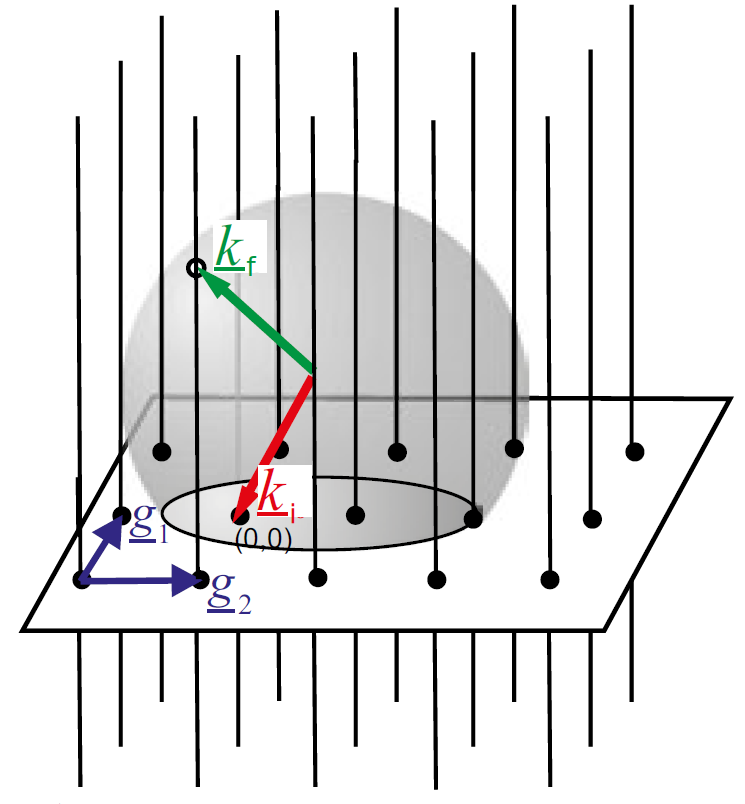
\includegraphics[width=0.4\textwidth]{Ewald}
            \caption{Schamtische darstellung zur Veranschaulichung der Konstruktion der Ewaldkugel.
            Blaue Pfeile stellen die reziproken Gittervektoren da. 
            Der rote Pfeil den einfallenden Wellenvektor der Elektronen, grün den der gestreuten.
            Kopiert und modifiziert aus~\cite{Fauster}.}
            \label{fig:Ewald}
        \end{figure}
        Die Beugungsreflexe lassen sich für nahezu senkrechten Einfall mit Hilfe der Ewaldkugel konstruieren, veranschaulicht zu sehen in \autoref{fig:Ewald}.
        Hierzu wird das reziproke Gitter aufgespannt, es ergeben sich auf Grund der gebrochenen Symmetrie Gitterstangen.
        Um einen beliebiegen Startpunkt wird eine Kugel mit dem Radius $\vec{k}_\text{i}$ gezeichnet, so ergeben sich für alle schneidenen Gitterstangen der Kugel auch Beugungsreflexe.
        Der Schnittpunkt mit der Kugel zum Ursprung hin ergibt dann den gebeugten Wellenzahlvektor $\vec{k}_\text{f}$.

        % Größere Abstände im Realraum werden im reziproken Raum kleiner abgebildet.
        % Mit steigeneder Energie der Elektronen rücken die Beugungsmaxima dichter zum Zentrum hin.
        Die Annahme ohne Mehrfachstreuung der Elektronen ist zu einfach gefasst, weswegen lange keine Strukturanalyse mittels LEED möglich war.
        Ursache der Mehrfachstreuung ist der verhältnissmäßig große Streuquerschnitt der langsamen Elektronen an Atomen.
        Es kommt vermehrt zur Streuung mit den nächsten Nachbarn der Primär- wie auch Sekundärwelle, die sich wiederum gegenseitig beeinflussen.
        Tendenziell ist es möglich aus der Position der Beugungsreflexe auf die Größe der Einheitszelle zu schließen, durch Adsorbate und Domänen, kann dies allerdings erschwert werden.
        Werden die Intensitäten der Spots durch Variation der Energie aufgezeichnet ergeben sich charakteristische IV-Kurven.
        Ihre theoretische Berechnung ist sehr aufwendig, da sie den Formfaktor und zahlreiche Streueffekte berücksichtigen müssen.
    
    \section{Augerelektronenspektroskopie} \label{sec:Auger}
        \begin{figure}
            \centering
            \includegraphics[width=0.4\textwidth]{Auger-Effekt.png}
            \caption{Schamtische Darstellung des Augerprozesses. Kopiert aus \cite{Auger-Bild}.}
            \label{fig:AES}
        \end{figure}
        Um sich die Zusammensetzung von Materialien genauer zu betrachten ist die Auger Methode eine einfache Methode.
        Der da hintersteckende Augerprozess wurde von L.~Meitner und P.~Auger unabhängig von einander im Jahre \num{1920} entdeckt \cite{Auger-Prozess}.
        Da die Atomorbitale für verschiedene Elements bei unterschiedlichen Energien liegen ist auch der Übergang zwischen zwei dieser Zustande eine charakteristische Energie.
        Für die Augerelektronenspektroskopie wird sich dieses von Nutzen gemacht.
        Hierfür muss zunächst ein Loch in einem der Kernniveaus erzeugt werden.
        Dies kann auf zwei verschiedene Arten geschehen.
        Eine ist in dem die Probe mit hochenergetischen Elektronen von eigenen Kilovolt beschossen werden und dabei ein Elektron herausschlägt.
        Dieser Prozess ist schematisch in \autoref{fig:AES} dargestellt.
        Die zweite Methode ist die Anregung mittels Photonen, welche dann ein Photoelektron auslösen.
        Dieser Prozess wird genauer in \autoref{sec:PES} behandelt.

        Nach dem Auslösen eines Elektrons befindet sich das Atom in einem angeregten Zustand.
        Um wieder eine energetisch günstigere Konfiguration einzunehmen muss ein Elektronen von einem energetisch niedrigerem Zustand (weiter außen liegend) das Loch auffüllen.
        Dabei kann die frei werdene Energie über ein Photon emittiert werden oder an ein weiteres Elektron abgegeben werden, dem Augerelektronen.
        Letzterer Prozess ist ebenfalls in \autoref{fig:AES} zu erkennen und beruht auf der Coulombwechselwirkung.
        Die kinetische Energie diese Elektrons ergibt sich dabei zu
        \begin{equation}
            E_\text{Kin} = E_\text{X} - E_\text{Y} -E_\text{Z} - \Delta U - \phi
        \end{equation}
        mit den Bindungsenergien des Zustandes in dem das Loch erzeugt wird $E_\text{X}$, des auffüllenden Elektrons $E_\text{Y}$ und dem emittierten Elektronen $E_\text{Z}$.
        Abgezogen werden muss noch die Austrittsarbeit $\phi$, welche der Energieunterschied zwischen der Fermienergie $E_\text{F}$ und der Vakuumenergie $E_\text{V}$ ist.
        Ferner muss noch eine Korrektur $\Delta U$ (meist klein) beachtet werden, da das Atom im zweifach ionisierten Zustand hinterlassen wird~\cite{Fauster}.
        Wie zuvor angemerkt ist diese Energiedifferenz charakteristisch für jedes Element.
        Werden die emittierten Elektronen auf ihre Energie hin untersucht.
        Dies kann zum einen durch ein weiteres Gitter in der LEED Optik geschehen, dann ist nur eine Elektronenkanone von Nöten.
        Andernfalls wird meist ein Zylinderspiegelanalysator verwendet, in dem die Elektronen nach ihrer Energie selektiert werden und anschließend vervielfältigt werden.
        Entsprechende Linien in Energie aufgelösten Spektren werden dabei einem Element und entsprechendem Übergang in der Röntgennotation mit Großbuchstaben (K, L, M) zugeordnet.
        Die Notataion setzt sich dabei aus den drei Buchstaben XYZ der Schalen zusammen, vobei das Valenzband durch den Buchstaben V ausgedrückt werden kann~\cite{Fauster}.

        Für die Auslösung eines Augerelektronens ist dabei maßgeblich die Wechselwirkungswahrscheinlichtkeit zwischen der verwendeten Anregung und entsprechendem Kernniveaus Auschlag gebend.
        Hinzukommt, dass für große Energiedifferenz der Prozess der Abregung durch Aussendung eine Photons, der Röntfluoreszenz dominiert wird.
        Für eine maximale Ausbeute sollten die anregenden Primärelektronen etwa dem dreifachen Bindungsenergie des Rumpfniveaus $E_\text{X}$ entsprechen~\cite{Fauster}.
        Dies kann zusammen gefasst werden in ein Sensetivitätsfaktor $S_i$ für entsprechendes Element.
        Entsprechende Werte für verschiedene Anregungen sind tabelliert~\cite{Auger}.
        Gemeinsam mit den Intensitäten $I_j$ der verschiedene Augerlinien im Spektrum kann anschließend die Konzentration einzelner Elemente
        \begin{equation}
            c_i = \frac{I_i/S_i}{\sum_j I_j/S_j}
            \label{eqn:Auger}
        \end{equation}
        der verschiedenen Bestandteile in der Probe bestimmt werden.
        Da die experimentell verwendeten kinetischen Energien im Bereich zwischen \SIrange[range-phrase=\:und\:]{100}{1200}{\electronvolt} lässt sich aus \autoref{fig:Weg} erkennen, dass diese Methode nicht immer Oberflächensensetiv ist.

    \section{Erweiterungen 2D Photoelektronen}
        Als Erweiterung der 2D Photoelektronen Mikroskopie sind auch zeitaufeglöste Messungen möglich.
        Hierbei erfolgt die Anregung mit zwei zeitlich versetzten Pulsen. 
        Dabei regt der erste Puls die Elektronen in einen höheren Zustand an und der zweite Puls löst diese dann aus.
        So ist es auch möglich zuvor unbesetzte Zustände (zwei Photonenemission) zu untersuchen.
        Wird der zeitliche Versatz zwischen den beiden Pulsen variiert so ist auch die Lebensdauer der Zustände abschätzbar.
        Für die gepulste Photonenquellen würde sich ein Flugzeit (TOF, \textit{Time of flight}) Analysator besser eignen.
        In einem TOF Analysators wird die kinetische Energie aus der Flugzeit der Elektronen bestimmt, weswegen es nur für gepulste Photonenquellen möglich ist.
        Der Vorteil liegt darin, dass direkt ein ganzer Datensatz für alle Impuls- und Energiewerte erfasst werden kann.

        Mögliche Erweiterung wäre auch die Elektronen nach der Energieselektion auch noch nach ihrem Spin zu sortieren.
        So lassen sich die magnetischen Eigenschaften genauer veranschaulichen.